\section*{Notices}

\subsection*{Emit notices}

\begin{itemize}
  \item[] \textbf{Trigger:} User interaction with CMS window
  \item[] \textbf{Precondition:} Assert that user has logged in
  \item[] \textbf{Path:}
    \begin{enumerate}
      \item User clicks Emit Notices on navigation bar
      \item User filters debts by filling up ``days in debt'' and ``amount'' and clicking in ``Refine search''
      \item User selects debts for the notice to be emitted
      \item User clicks ``Emit Notices''
      \item ``Notices have been emitted'' message is shown
    \end{enumerate}
  \item[] \textbf{Requirements:}
    \begin{enumerate}
      \item Email are sent to the tenants in debt with information about the outstanding debts
      \item The debts selected are marked as notified
    \end{enumerate}
  \item[] \textbf{Screenshots:} \\
    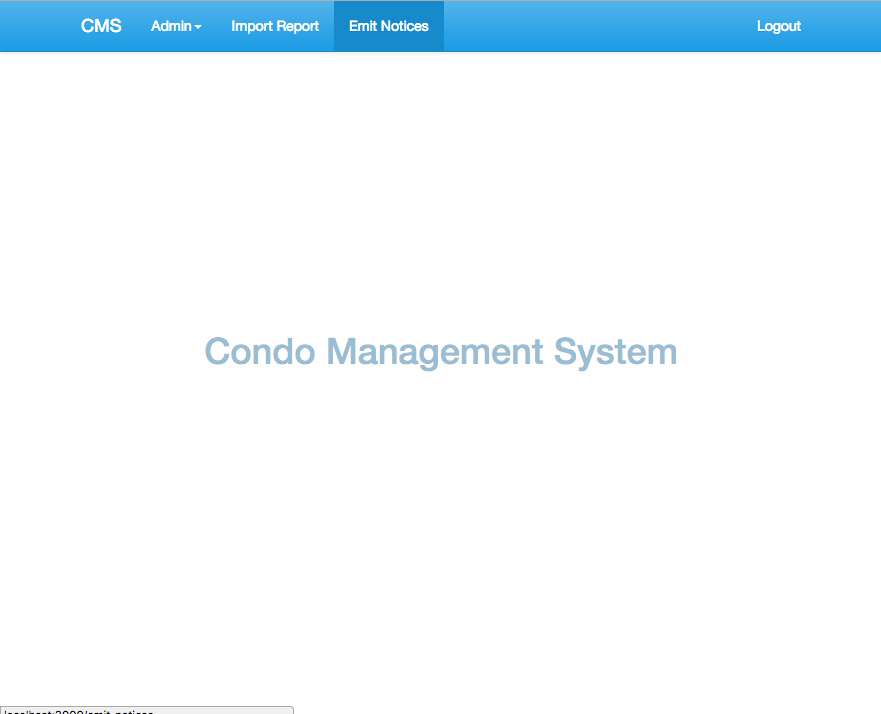
\includegraphics[scale=0.25]{./images/ss/notice/1.png}
    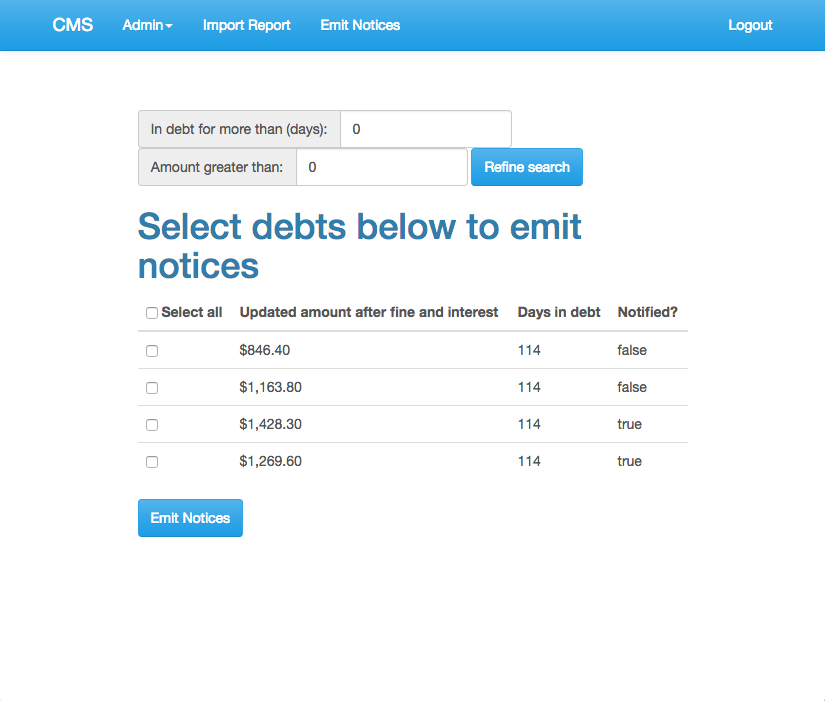
\includegraphics[scale=0.25]{./images/ss/notice/2.png}\\
    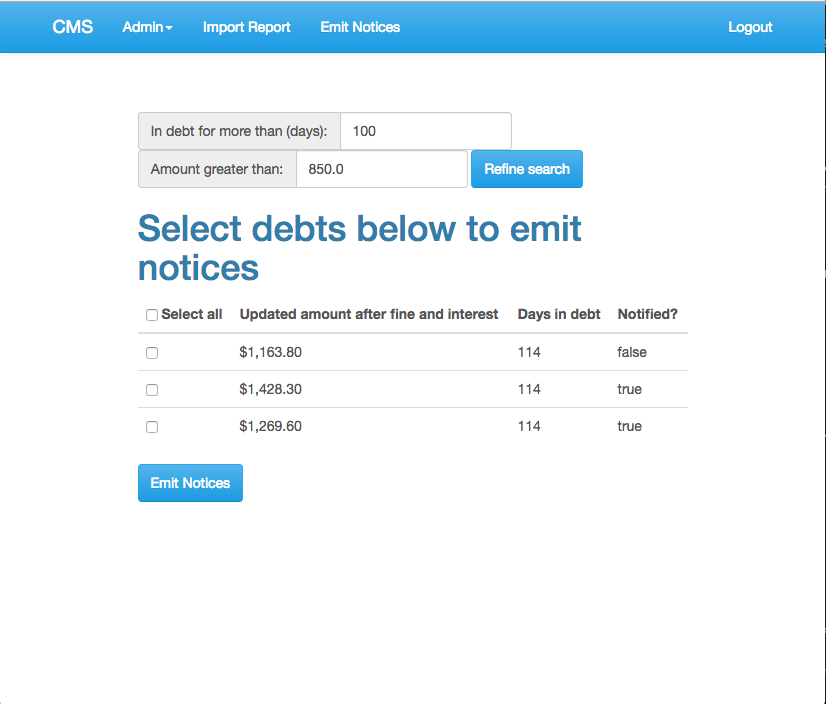
\includegraphics[scale=0.25]{./images/ss/notice/3.png}
    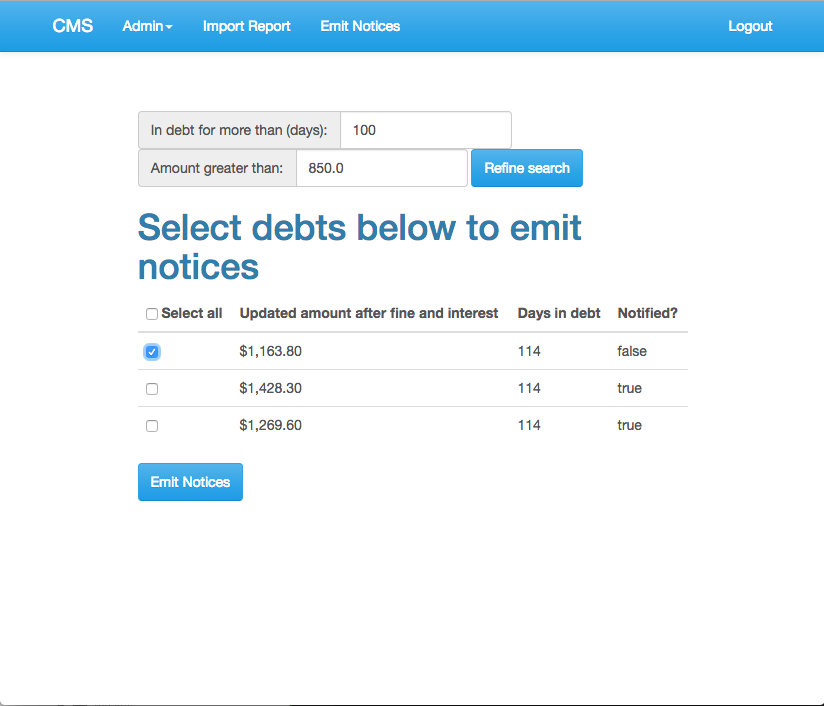
\includegraphics[scale=0.25]{./images/ss/notice/4.png}\\
    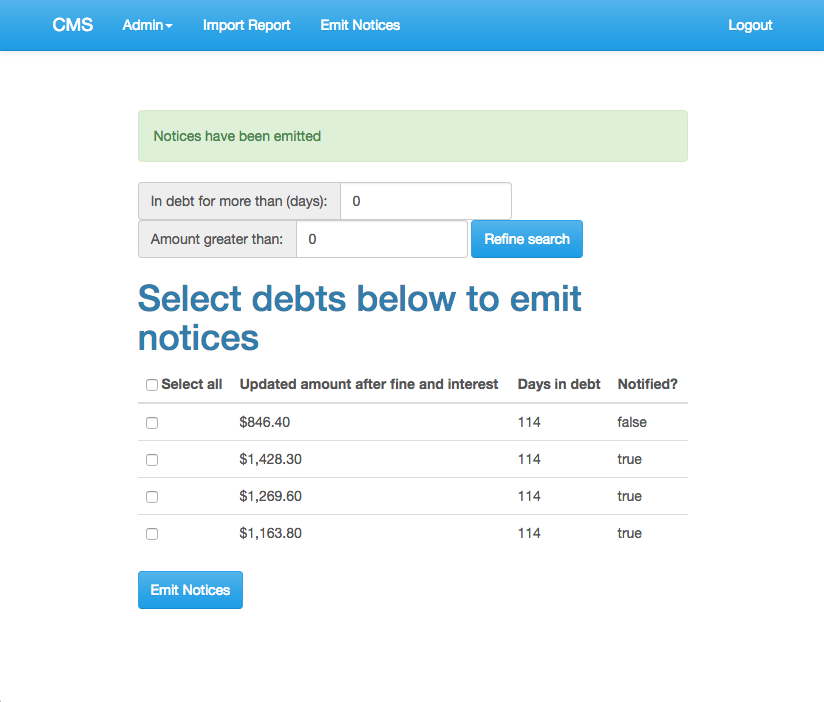
\includegraphics[scale=0.25]{./images/ss/notice/5.png}
\end{itemize}
